
\chapter{Treatment of experimental uncertainties}
\label{C:treatm-exper-uncert}


\section{Introduction}\label{S:Intro}

The cross sections of interest are related by
\[
\frac{d \sigma}{d \Omega_{P} d E_{e} d \Omega_{e}} \approx (M_{P} v)^{2} \,\frac{d \sigma}{d \bm{Q} d E_{e} d \Omega_{e}} = \frac{(M_{P} v)^{2}}{2 \pi Q} \,\frac{d \sigma}{d Q d E_{e} d \Omega_{e}}
\]
%
or, equivalently:
%
\[
\frac{d \sigma}{d \Omega_{P} d E_{e} d \Omega_{e}} \approx (M_{P} v)^{2} \,\frac{d \sigma}{d \bm{Q}_{\perp} d E_{e} d \Omega_{e}} 
\]
if we evaluate the right hand side of these equations at $Q= \sqrt{Q_{\perp}^{2}+ (\Delta E_{e}/v)^{2}}$

\section{Approximations}
\label{S:approx}

We have analyzed different flavors of CDW. Figures \ref{F:comparac3} and \ref{F:comparacdw} show different descriptions of the initial and final states in CDW-B1 and CDW-EIS approximations. Strangely enough the approximation that best fits the experimental data is the one that completely neglects the internuclear interaction. 

\begin{figure}[!htpb]
  \label{F:comparac3}
  \centering
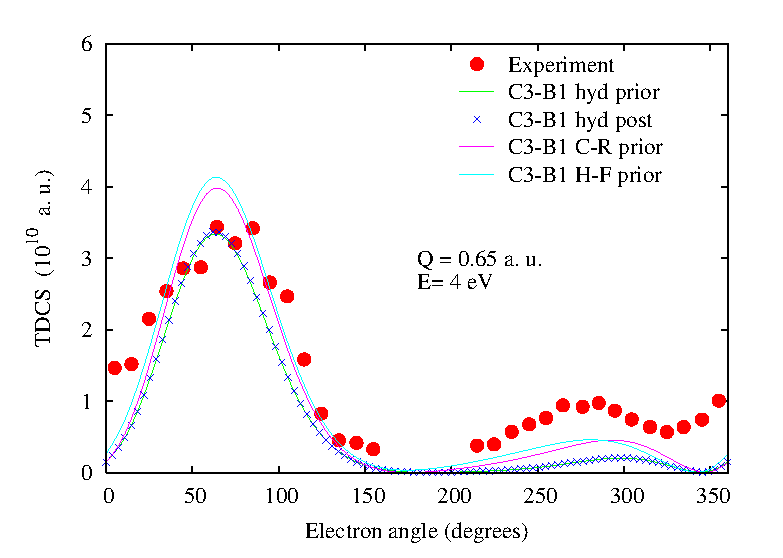
\includegraphics[width=0.7\textwidth]{compara_c3}
  \caption{TDCS for $E_{e}=4$ eV and $Q=0.65$~a.u. in the CDW-B1 approximation for different representation of the initial and final states.}
\end{figure}

\begin{figure}[!htpb]
  \label{F:comparacdw}
  \centering
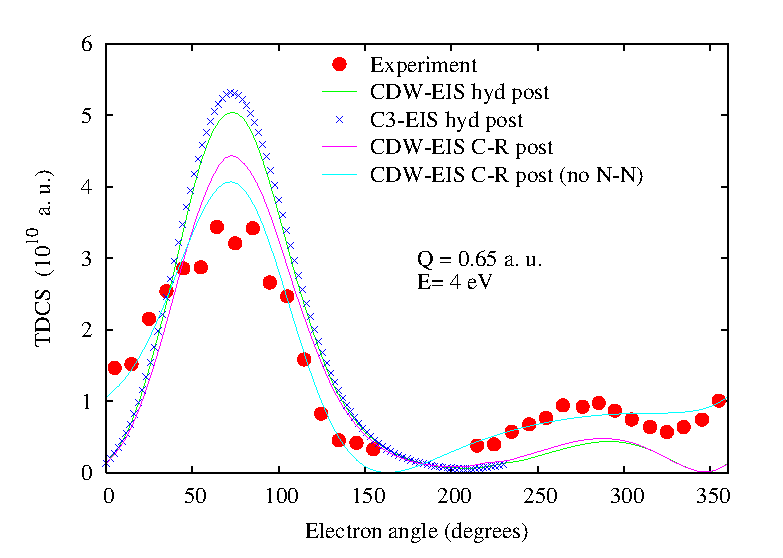
\includegraphics[width=0.7\textwidth]{compara_cdw}
  \caption{TDCS for $E_{e}=4$ eV and $Q=0.65$~a.u. in the CDW-EIS approximation for different representation of the initial and final states.}
\end{figure}

\section{Effective charge dependency}
\label{S:effec-charg-depen}

In the CDW-EIS approximation we studied the effect of the nuclear-nuclear interaction. We described it as a Coulomb force of charge ZN. As observed before, the best description is given for negligible internuclear interaction. 

\begin{figure}[!htpb]
  \centering
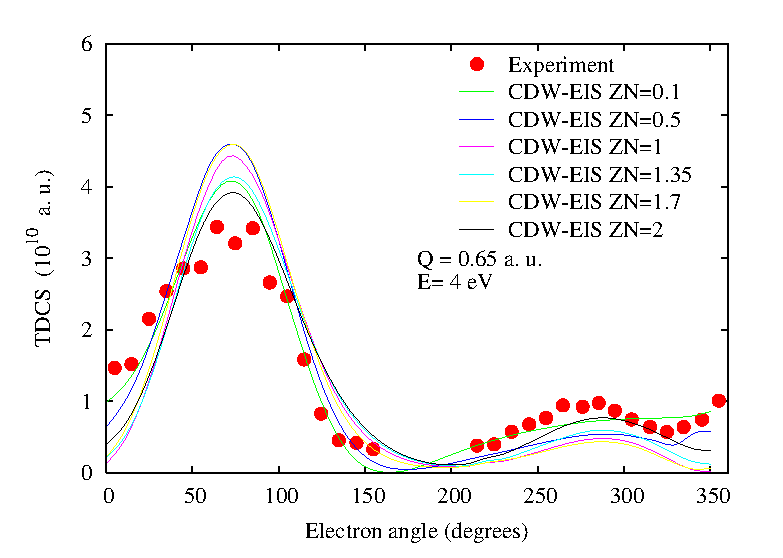
\includegraphics[width=0.7\textwidth]{compara_cdwZN}
  \caption{TDCS for $E_{e}=4$ eV and $Q=0.65$~a.u. in the CDW-EIS approximation for different charges of the internuclear interaction.}
  \label{F:compara-cdwZN}
\end{figure}


\section{Inclusion of experimental uncertainties}
\label{S:inclu-exper-uncer}

Here we want to discuss how to do the convolution over the temperature. The result is very different if we convolute the cross section
${d \sigma}/{d \Omega_{P} d E_{e} d \Omega_{e}}$ or $ {d \sigma}/{d \bm{Q} d E_{e} d \Omega_{e}} $ because the factor $1/Q$ that relates them gives different weights to cross sections for small and large $Q$ in each case.

The main assumption is that the target atom in the initial state is not at rest but has a random momentum $K_{i}$ with probability given by a Gauss distribution in each direction
\begin{equation}\label{Q:gauss-distr}
 p(K_{i}) dK_{i} = \frac{1}{\sqrt{2 \pi \sigma_{i}^2}} \exp (-K_{i}^{2} / 2\sigma_{i}^{2}) dK_{i} \, .  
\end{equation}
%
 The standard deviation $\sigma$ is related to the jet temperature by $\sigma=\sqrt{M_{T} k_{B} T}$, where $k_{B}$ is Boltzmann's constant. This relation gives $\sigma = 0.15$~a.u. for $T=1^{\circ}$K.

If we consider negligible the uncertainty in the determination of the electron momentum $\bm{k}$, we can carry the uncertainty in the atom initial momentum over to the momentum transfer $\bm{Q}=\bm{K}_{R}+ \bm{k}$

Thus, in the case of perfect experimental conditions for the electron, the experimental cross section is determined from the number of events such that the  momentum of the recoil is $\bm{K}_{R}=\bm{Q}+\bm{k}$. The observed cross section for a nominal momentum transfer $\bm{Q}_{0}$ is obtained from the convolution over the uncertainties:

\[
\frac{d \sigma}{d \bm{Q}_{0} d E_{e} d \Omega_{e}} = \int_{\Delta \bm{Q}} \frac{d \sigma}{d \bm{Q} d E_{e} d \Omega_{e}}\, p( \bm{Q} - \bm{Q}_{0} ) \, d \bm{Q}
\]

Now, let's consider that the two perpendicular components present the same uncertainty while the perpendicular is perfectly determined (much smaller deviation $\sigma$ in real life). Then, the two-dimensional distribution can be rewritten for the magnitude of the perpendicular component and one angle


\begin{eqnarray*}
  p(\bm{Q}_{\perp} - \bm{Q}_{{\perp},0}) d\bm{Q}_{\perp} &=&  p(Q_{x}-Q_{x,0}) dQ_{x} \, p(Q_{y}-Q_{y,0}) d Q_{y} \\
&=& \frac{1}{2 \pi \sigma^2} \, \exp \left[{- \left|\bm{Q}_{\perp} - \bm{Q}_{{\perp},0}\right|^{2} / 2\sigma^{2}} \right] Q_{\perp} \, dQ_{\perp} \, d \varphi_{Qe} \, .
\end{eqnarray*}



In conclusion, we have to add the experimental results in the following way

\begin{align}\label{Q:convol-exact}
 \frac{d \sigma}{d \bm{Q}_{\perp , 0} d E_{e} d \Omega_{e}} &= \int_{\Delta \bm{Q}} \frac{d \sigma}{d \bm{Q}_{\perp} d E_{e} d \Omega_{e}}\, p( \bm{Q}_{\perp} ) \, d \bm{Q}_{\perp} \nonumber \\
&= \frac{1}{2 \pi \sigma^{2}} \int_{0}^{\infty} Q_{\perp} \, d Q_{\perp} \int_{0}^{2 \pi}  \frac{d \sigma}{ d \bm{Q}_{\perp} d E_{e} d \Omega_{e}}\, e^{- \left|\bm{Q}_{\perp} - \bm{Q}_{{\perp},0}\right|^{2} / 2\sigma^{2}} \, d \varphi_{Q_{\perp}} \nonumber \\
&= \frac{1}{2 \pi \sigma^{2}} \int_{0}^{\infty} e^{- \left({Q}^{2}_{\perp} + {Q}^{2}_{{\perp},0}\right)^{2} / 2\sigma^{2}}  Q_{\perp} \, d Q_{\perp} \int_{0}^{2 \pi}  \frac{d \sigma}{ d \bm{Q}_{\perp}}\, e^{{Q}_{\perp} {Q}_{{\perp},0} \cos{\varphi}/\sigma^{2}} \, d \varphi_{Q_{\perp}}
\nonumber \\
&= \frac{e^{- Q^{2}_{{\perp},0} / 2\sigma^{2}} } {\sqrt{2 \pi \sigma^{2}}} \int_{0}^{\infty}   \frac{e^{- Q^{2}_{{\perp}} / 2\sigma^{2}} } {\sqrt{2 \pi \sigma^{2}}} \, Q_{\perp} d Q_{\perp} \int_{0}^{2 \pi}  \frac{d \sigma}{ d \bm{Q}_{\perp}}\, e^{{Q}_{\perp} {Q}_{{\perp},0} \cos{\varphi}/\sigma^{2}} \, d \varphi_{Q_{\perp}}
\nonumber \\
&= 2\, p(Q_{\perp,0},\sigma) \int_{0}^{\infty}  p(Q_{\perp},\sigma) \, Q_{\perp} d Q_{\perp} \int_{0}^{\pi}  \frac{d \sigma}{ d \bm{Q}_{\perp}}\, e^{{Q}_{\perp} {Q}_{{\perp},0} \cos{\varphi}/\sigma^{2}} \, d \varphi_{Q_{\perp}} 
\end{align}
%
where $p(x,\sigma)$ is the Gauss distribution of Eq. \ref{Q:gauss-distr}.



\subsection*{Peaking approximation at $\varphi=0$}

Now, the roughest approximation for the integral on the azimuthal angle $\varphi$ would be to consider that the cross section is independent of it and take it out of the integral. In this way we obtain

\begin{eqnarray}\label{Q:Aprox-0-convo}
\frac{d \sigma}{d \bm{Q}_{\perp , 0} d E_{e} d \Omega_{e}} 
&=& p(Q_{\perp,0},\sigma) \int_{0}^{\infty}  p(Q_{\perp},\sigma) \, \left(Q_{\perp} \frac{d \sigma}{ d \bm{Q}_{\perp}}(Q_{\perp})\right)_{\varphi=0} \, d Q_{\perp} \int_{0}^{2 \pi} \, e^{{Q}_{\perp} {Q}_{{\perp},0} \cos{\varphi}/\sigma^{2}} \, d \varphi_{Q_{\perp}} 
\nonumber \\
&=& p(Q_{\perp,0},\sigma) \int_{0}^{\infty}  p(Q_{\perp},\sigma) \, \left(Q_{\perp} \frac{d \sigma}{ d \bm{Q}_{\perp}}(Q_{\perp})\right)_{\varphi=0} \, d Q_{\perp} \left[ 2 \pi \,I^{B}_{0}(Q_{\perp} Q_{\perp,0}/\sigma^{2}) \right]
\end{eqnarray}
%
where $I^{B}_{0}$ is the Modified Bessel function (see chapter 9, page 376 of \cite{Abramow1972_HOM}).


\begin{figure}[!htpb]
  \centering
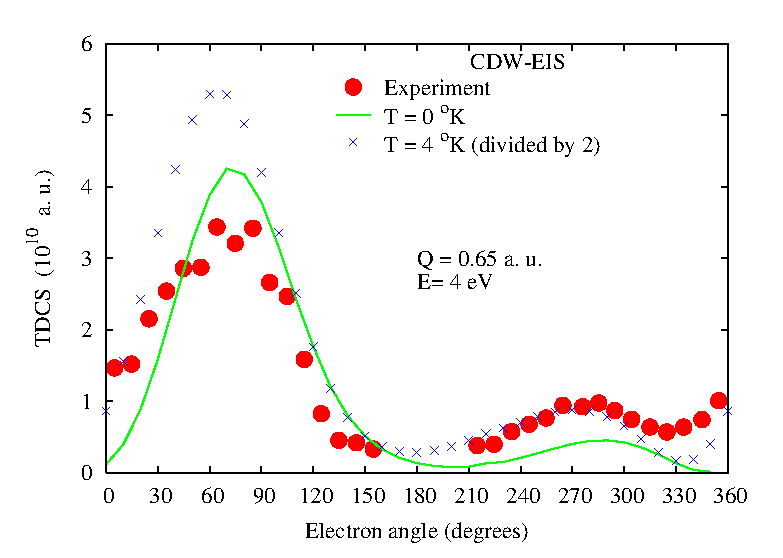
\includegraphics[width=0.7\textwidth]{cdwe4q065t4_app0}
  \caption{TDCS for $E_{e}=4$ eV and $Q=0.65$~a.u. in the CDW-EIS approximation for temperature convolution in approximation 0.}
  \label{F:cdwe4q065t4_app0}
\end{figure}


\subsection*{Peaking approximation at $\varphi=0$ and $\varphi=\pi$}

The next level of approximation would be to consider separately the coplanar $(\varphi=0)$ and anti-coplanar $(\varphi=\pi)$ directions.

\begin{flalign}\label{Q:Aprox-1-convo}
 \frac{d \sigma}{d \bm{Q}_{\perp , 0} d E_{e} d \Omega_{e}} =&
 p(Q_{\perp,0},\sigma) \int_{0}^{\infty}  p(Q_{\perp},\sigma) \, d Q_{\perp} \times 
\\
& \left[ \left( 2 \pi Q_{\perp} \frac{d \sigma}{ d \bm{Q}_{\perp}} \right)_{\varphi=0} \, \,I_{0} \left( \frac{Q_{\perp} Q_{\perp,0}}{\sigma^{2}} \right) + 
 \left( 2 \pi Q_{\perp} \frac{d \sigma}{ d \bm{Q}_{\perp}} \right)_{\varphi=\pi} \,I_{0}\left( -\frac{Q_{\perp} Q_{\perp,0}}{\sigma^{2}} \right)\right] \nonumber
\end{flalign}
%
where we have defined 

\begin{equation}\label{Q:I0}
  I_{0}(x)= \frac{1}{\pi} \, \int_{0}^{\pi/2} e^{x \, \cos(\varphi)} \, d \varphi
\end{equation}
%
such that $I^{B}_{0}(x) = I_{0}(x) + I_{0}(-x)$.


\begin{figure}[!htpb]
  \centering
\includegraphics[width=0.7\textwidth]{cdwe4q065t4_app1}
  \caption{TDCS for $E_{e}=4$ eV and $Q=0.65$~a.u. in the CDW-EIS approximation for temperature convolution in approximation 0.}
  \label{F:cdwe4q065t4_app1}
\end{figure}

The virtue of these approximations is that not out-of-the-plane calculations are needed.


\subsection{Anisotropic resolution in cylindrical coordinates}
\label{S:anis-resol-cylin-coord}

Sebasti\'{a}n derived the following expresion for $\sigma_{x}\neq \sigma_{y}$

\[
\left\langle \frac{d \sigma }{dQ_{\perp}} \right\rangle = \frac{1}{2\pi
  \sigma_{x} \sigma_{y}} \int_{0}^{\infty} dQ_{\perp} \int_{0}^{\pi} d\varphi
\left(p (Q_{\perp },\varphi ,Q_{0\perp}) + p(Q_{\perp },2\pi -\varphi
  ,Q_{0\perp}) \right)
\]

\begin{eqnarray*}
  p(Q_{\perp },\varphi ,Q_{0}) &=&\exp \left[ -\frac{(Q_{\perp }^{2}\cos
      ^{2}\varphi +Q_{0\perp }^{2}\cos ^{2}\varphi _{0}-2Q_{\perp }Q_{0\perp }\cos
      \varphi \cos \varphi _{0})}{2\sigma _{x}^{2}} \right] 
  \\
  && \left.  - \frac{(Q_{\perp }^{2} \sin^{2}\varphi +Q_{0\perp }^{2}\sin ^{2}\varphi _{0}-2Q_{\perp }Q_{0\perp }\sin
      \varphi \sin \varphi _{0})}{2\sigma _{y}^{2}}\right]  \\
  p(Q_{\perp },2\pi -\varphi ,Q_{0}) 
  &=&\exp \left[ - \frac{(Q_{\perp }^{2}\cos^{2} \left( 2\pi -\varphi \right) +Q_{0\perp }^{2} \cos ^{2}\varphi_{0} - 
      2Q_{\perp }Q_{0\perp }\cos \left( 2\pi -\varphi \right) \cos \varphi_{0})} {2\sigma_{x}^{2}} \right.  \\
  && \left. - \frac{(Q_{\perp }^{2}\sin ^{2}\left( 2\pi -\varphi \right) + Q_{0\perp }^{2}\sin ^{2}\varphi _{0}-2Q_{\perp }Q_{0\perp } 
      \sin\left( 2\pi -\varphi \right) \sin \varphi _{0})}{2\sigma _{y}^{2}}\right] 
\end{eqnarray*}

If $\sigma_{x} = \sigma_{y}=\sigma $ then these last expressions reduce to,

\begin{eqnarray*}
p(Q_{\perp },\varphi ,Q_{0}) &=&\exp \left[ -\frac{(Q_{\perp }^{2}+Q_{0\perp}^{2}-2Q_{\perp} Q_{0\perp }\cos \varphi \cos \varphi _{0}-2Q_{\perp} Q_{0\perp }\sin \varphi \sin \varphi _{0})}{2\sigma ^{2}}\right]  \\
p(Q_{\perp },2\pi -\varphi ,Q_{0}) &=&\exp \left[ -\frac{(Q_{\perp}^{2}+Q_{0\perp }^{2}-2Q_{\perp }Q_{0\perp }\cos \left( 2\pi -\varphi \right) \cos \varphi _{0}-2Q_{\perp }Q_{0\perp }\sin \left( 2\pi -\varphi \right) \sin \varphi _{0})}{2\sigma ^{2}}\right] 
\end{eqnarray*}


\subsection{Anisotropic resolution in cartesian coordinates} 
\label{S:anis-resol-carte-coord}

Starting from the general expresion for a gaussian uncertainty in the momentum
\[
\frac{d \sigma}{d \bm{Q}_{0} d E_{e} d \Omega_{e}} = \int_{\Delta
  \bm{Q}} \frac{d \sigma}{d \bm{Q} d E_{e} d \Omega_{e}}\, p_{x}( Q_{x}- Q_{0,x} ) p_{y}( Q_{y}- Q_{0,y} ) \, d Q_{x} d Q_{y}
\]
with
\[
 p_{i}(K_{i}) dK_{i} = \frac{1}{\sqrt{2 \pi \sigma_{i}^2}} \exp (-K_{i}^{2} / 2\sigma_{i}^{2}) dK_{i} \, .  
\]

In order to perform these convolutions we will integrate numerically these expresions interpolating the cross sections using splines in one direction and taking the average of the values in the other. A good check will be to choose first one and then the other direcion for the interpolation.

\subsection{Results for exact convolution}
\label{S:resul-exact-convol}

These are the results obtained with the two-dimensional integral in the angle $\varphi$ and the momentum transfer $Q_{\perp}$ given by (\ref{Q:convol-exact}), using a Simpson routine with step $\Delta \varphi = 10^{\circ}$ and $\Delta Q_{\perp}=0.05$ for $0.05 \le Q_{\perp} \le 1.55$~a.u.  The use of a Simpson routine . 

\begin{figure}[!htpb]
  \centering
\includegraphics[width=0.7\textwidth]{cdwe4q065t4_app2}
  \caption{TDCS for $E_{e}=4$ eV and $Q=0.65$~a.u. in the CDW-EIS approximation for temperature convolution with T$=4^{\circ}$K.}
  \label{F:cdwe4q065t4_app2}
\end{figure}

\begin{figure}[!htpb]
  \centering
\includegraphics[width=0.7\textwidth]{cdwe4q065t4_app2_125}
  \caption{TDCS for $E_{e}=4$ eV and $Q=0.65$~a.u. in the CDW-EIS approximation for temperature convolution, scaled by 1.25.}
  \label{F:cdwe4q065t4_app2_125}
\end{figure}

These calculations were performed with $Z_{N}=1.354$ though the impact parameter dependence observed for the CTMC seems to indicate that $Z_{N}=1$ is more adequate.  As observed in figure \ref{F:compara-cdwZN} the binary peak is slightly higher for $Z_{N}=1.0$. 


%%% Local Variables: 
%%% mode: latex
%%% TeX-master: "main"
%%% End: 
